\section{Applied 2016: Solution \footnote{Gene Katsevich, Kenneth Tay, Stephen Bates, Nikos Ignatiadis, Isaac Gibbs, Dan Kluger and M.H.}}

\subsection*{Problem 1: Quadratic discriminant analysis and EM}
Key ideas/tools:
\begin{itemize}
\item LDA and QDA as Gaussian mixture models
\item using EM for semi-supervised learning.
\end{itemize}


Let $y = 1$ denote ``otic" cells and $y = 0$ denote non-otic cells.

\begin{itemize}
\item[(a)] From the left plot, we see that the two Gaussian distributions have different means and covariance matrices. Hence, we can posit the following generative model:
	\begin{equation}
	\begin{split}
	&y_i \simiid \text{Ber}(\pi); \\
	&x_i|y_i=k \sim \mathcal N(\mu_k, \Sigma_k), \quad k = 0, 1. 
	\end{split}
	\end{equation}
	To fit these parameters, we can use maximum likelihood, for $k=0,1$,
	\begin{align}
	\hat \pi &= \frac{1}{n}\sum_{i = 1}^n y_i,\nonumber  \\
	 \hat \mu_k &= \frac{\sum_{i = 1}^n x_i I(y_i = k)}{\sum_{i = 1}^n I(y_i = k)},\nonumber  \\
	  \hat \Sigma_k &= \frac{\sum_{i = 1}^n (x_i-\hat \mu_k)(x_i - \hat \mu_k)^\top  I(y_i = k)}{\sum_{i = 1}^n I(y_i = k)}.
	\label{parameter_estimates}
	\end{align}
	Based on these fitted parameters, we can classify a point $x$ as otic if
	\begin{equation}
	\log \frac{\hat{\mathbb P}[y = 1|x]}{\hat{\mathbb P}[y = 0|x]} > 0,
	\label{decision}
	\end{equation}
	where $\hat{\mathbb{P}}$ is the probability distribution under the parameters $\hat{\pi}, \hat{\mu}_k$ and $\hat{\Sigma}_k$. This is quadratic discriminant analysis (QDA).
\item[(b)]  We have by Bayes' rule
	\begin{align}
	\log \frac{\mathbb P[y = 1|x]}{\mathbb P[y = 0|x]} &= \log\left(\frac{\pi}{1-\pi}\frac{\phi_{\mu_1, \Sigma_1}(x)}{\phi_{\mu_0, \Sigma_0}(x)}\right) \nonumber \\
	&= \log\left(\frac{\pi}{1 - \pi}\right) -\frac12 \log |\Sigma_1| - \frac{1}{2}(x - \mu_1)^\top  \Sigma_1^{-1}(x - \mu_1) \nonumber \\ &\qquad+ \frac12 \log |\Sigma_0| + \frac{1}{2}(x - \mu_0)^\top  \Sigma_0^{-1}(x - \mu_0). \label{log_odds}
	\end{align}
This quantity is a quadratic form in $x$, so we get a quadratic decision boundary. 

\item[(c)] I would take the parameter estimates from (\ref{parameter_estimates}) and plug them into the log-odds expression (\ref{log_odds}) together with the $x$ value of the new data point. Having calculated this log odds, I would classify the point based on (\ref{decision}).

\item[(d)] Intuitively, the unlabeled data carries information about $\mu_k$ and $\Sigma_k$. However, we cannot directly use these unlabeled data points without assigning them to classes. To address this problem, we can treat these unknown class labels as missing data, and estimate all the parameters with maximum likelihood estimation by using the EM algorithm. In the E step, we need to calculate the probability 
	\begin{equation}
	\mathbb P[z = 1|x, \pi^{(t)}, \mu_k^{(t)}, \Sigma_{k}^{(t)}].
	\end{equation}
	This is a calculation similar to (\ref{log_odds}). In the M step, we would plug these ``soft assignments" to calculate the expected complete-data likelihood and maximize with respect to the parameters. One way of initializing the EM algorithm is with the parameter estimates obtained from just the labeled data. 
	
	
	While the problem states ``briefly sketch how" and simply mentioning the above could suffice, if there is time on the exam it is worth sketching out in more detail how you would implement the EM algorithm. Let $N_l$, denote the number of labeled samples and $N_u$ denote the number of unlabeled samples $y_1,\dots, y_{N_l}$ are observed indicators of whether each labeled cell is otic and let $Z_{N_l+i}$ for $1 \le i \le N_u$ be the unobserved latent variable indicating whether or not the cell is otic. Note that our model for the data is,
\begin{align*}
y_i&\simiid \text{Ber}(\pi), \\
Z_i &\simiid  \text{Ber}(\pi),\\
 x_i|y_i=k &\sim \mathcal N(\mu_k, \Sigma_k), \\ 
 x_i|Z_i=k &\sim \mathcal N(\mu_k, \Sigma_k)
\end{align*}
	Letting $\theta= (\pi, \mu_0,\Sigma_0,\mu_1,\Sigma_1)$ denote the parameter of the model, and observe that the log-likelihood is given by 
$$\begin{aligned}
&\ell(\theta;X,Y) \\
& =\sum_{i=1}^{N_l} y_i \Big( \log(\pi)+ \log \big( \phi_{\mu_1, \Sigma_1}(x_i) \big) \Big)+(1-y_i) \Big( \log(1- \pi) +\log \big( \phi_{\mu_0, \Sigma_0}(x_i) \big) \Big) \\
& +\sum_{i=N_l+1}^{N_l+N_u}   \log \big( \pi \phi_{\mu_1, \Sigma_1}(x_i)  + (1-\pi) \phi_{\mu_0, \Sigma_0}(x_i) \big)
\end{aligned}$$

We seek to find the $\hat{\theta}$ maximizing the above expression. This can be done by using the EM algorithm, by noting that the complete log likelihood is given by 

$$\begin{aligned}
&\ell_c(\theta;X,Y,Z)\\
 & =\sum_{i=1}^{N_l} y_i \Big( \log(\pi)+  \log \big( \phi_{\mu_1, \Sigma_1}(x_i) \big) \Big)+(1-y_i) \Big( \log(1- \pi) + \log \big( \phi_{\mu_0, \Sigma_0}(x_i) \big) \Big) \\
& +\sum_{i=N_l+1}^{N_l+N_u}  Z_i \Big( \log(\pi)+ \log \big( \phi_{\mu_1, \Sigma_1}(x_i) \big) \Big)+ (1-Z_i) \Big( \log(1-\pi) + \log \big( \phi_{\mu_0, \Sigma_0}(x_i) \big) \Big).
\end{aligned}$$

To implement the E-step for each $\hat{\theta},i$ define $\gamma_{\hat{\theta},i} = y_i$ if $i \in \{1,\dots,N_l \}$ and define 
\begin{align*}
	\gamma_{\hat{\theta},i} &:=\mathbb{E}_{\hat{\theta}} [Z_i |X,Y]\\
	& =\mathbb{P}_{\hat{\theta}} [Z_i=1|x_i] \\
	&= \frac{\hat{\pi} \phi_{\hat{\mu}_1, \hat{\Sigma}_1}(x_i) }{\hat{\pi} \phi_{\hat{\mu}_1, \hat{\Sigma}_1}(x_i)+(1-\hat{\pi}) \phi_{\hat{\mu}_0, \hat{\Sigma}_0}(x_i)}
\end{align*} 
For $N_l < i \leq N_l+N_u,$. The expected complete log-likelihood conditional on the observed data is given by
\begin{align}\label{eq:EStep}
&\mathbb{E}_{\hat{\theta}} \big[l_c(\theta;X,Y,Z) \big| X,Y \big] \nonumber \\
&= \sum_{i=1}^{N} \gamma_{\hat{\theta},i} \Big( \log(\pi) + \log \big( \phi_{\mu_1, \Sigma_1}(x_i) \big) \Big) + \Big( \log(1-\pi)  +   (1-\gamma_{\hat{\theta},i}) \log \big( \phi_{\mu_0, \Sigma_0}(x_i) \big) \Big),
\end{align}
where $N =N_l+N_u$.

To implement the M-step, note that the above objective is separable in $\pi$, $(\mu_0,\Sigma_0)$ and $(\mu_1,\Sigma_1)$. By taking the derivative with respect to $\pi$ setting to $0$ and by taking the gradients with respect to $(\mu_k,\Sigma_k)$ for $k=0,1$ and setting to zero,

$$\pi^{(t+1)} = \frac{1}{N} \sum_{i=1}^N \gamma_{\theta^{(t)},i}, \quad \mu_1^{(t+1)} = \frac{ \sum_{i=1}^N \gamma_{\theta^{(t)},i} x_i}{\sum_{i=1}^N  \gamma_{\theta^{(t)},i}  } , \quad \mu_0^{(t+1)} = \frac{\sum_{i=1}^N (1- \gamma_{\theta^{(t)},i} ) x_i}{\sum_{i=1}^N (1- \gamma_{\theta^{(t)},i} ) },$$
and 
\begin{align*} 
	\Sigma_1^{(t+1)}&= \frac{\sum_{i=1}^N \gamma_{\theta^{(t)},i} (x_i - \mu_1^{(t+1)})(x_i -\mu_1^{(t+1)})^\top  }{\sum_{i=1}^N  \gamma_{\theta^{(t)},i}  },\\
	  \Sigma_0^{(t+1)} &= \frac{\sum_{i=1}^N (1-\gamma_{\theta^{(t)},i}  )(x_i - \mu_0^{(t+1)})(x_i -\mu_0^{(t+1)})^\top }{\sum_{i=1}^N (1- \gamma_{\theta^{(t)},i} ) }.
\end{align*}
Note that solving for $\Sigma_k^{(t+1)}$ in the M-step is a bit tricky and can be done using formulas (57) and (61) in the Matrix cookbook. To find the maximum likelihood you alternate between the E-step and M-step updating $\hat{\theta} =\theta^{(t+1)}$. As mentioned earlier one good way to initialize the EM algorithm here is to use the estimates from part (a).
\end{itemize}


% Problem 2
\subsection*{Problem 2: Three angles and measurement error}

Key ideas/tools:
\begin{itemize}
\item writing down a model
\item maximum likelihood estimation
\end{itemize}


We find that the angles do not add up exactly to 180$^\circ$. The problem is that these angles contain measurement error.

In order to estimate the true angles, we must postulate a probability model for the measurement error. If the measurements are $y_1, y_2, y_3$ and the true angles are $\theta_1, \theta_2, \theta_3$, then the simplest model for measurement error is
\begin{equation}
y_i = \theta_i + \eps_i, \quad \eps_{i} \overset{\text{i.i.d.}}\sim \mathcal N(0, \sigma^2).
\end{equation}
Assuming a constant error variance would be problematic if the angles were very different in size (e.g. if one of the angles was $1^\circ$), but in our case it seems reasonable. We have the additional constraint that $\theta_1 + \theta_2 + \theta_3 = 180$, so we can parameterize the problem using $(\theta_1, \theta_2)$ only. Hence, we can estimate these two parameters from the following linear regression:
\begin{equation}
\left( \begin{array}{c}
y_1 \\
y_2 \\
y_3 - 180 \end{array} \right)= \left( \begin{array}{cc}
1 & 0 \\
0 & 1\\
-1 & -1 \end{array} \right)\left( \begin{array}{c}
\theta_1 \\
\theta_2 \end{array} \right) + \left( \begin{array}{c}
\eps_1 \\
\eps_2 \\
\eps_3 \end{array} \right). 
\end{equation}
Then, $(\hat \theta_1, \hat \theta_2, 180 - \hat \theta_1 - \hat \theta_2)$ would be our best guess for the true angles (these should also satisfy the constraints of positive angles, otherwise we could incorporate the constraints into the least squares optimization). The OLS estimate ends up being 
\begin{align*}
	\begin{bmatrix}
		\hat{Y}_1 \\ \hat{Y}_2 \\ \hat{Y}_3
	\end{bmatrix} &= \begin{bmatrix}
		\frac{2}{3}Y_1 - \frac{1}{3}(Y_2+Y_3) + 60^\circ\\
		\frac{2}{3}Y_2 - \frac{1}{3}(Y_1+Y_3) + 60^\circ\\
		\frac{2}{3}Y_3 - \frac{1}{3}(Y_1+Y_2) + 60^\circ
	\end{bmatrix}
\end{align*}


% Problem 3
\subsection*{Problem 3: A missing species problem}
Key ideas/tools:
\begin{itemize}
\item mixture models
\item Empirical Bayes
\end{itemize}

\paragraph{Context:} \citet{efron2016empirical} proposes empirical Bayes estimation in which the prior is specified as a flexible exponential family. Estimation can proceed parametrically by maximum likelihood. I think the question is not worded very clearly and may be interpreted in multiple ways depending on how you interpret the description of the distribution of $X_i$. Below we just present one interpretation.

\begin{itemize}
\item[(a)] We have
	\begin{equation}
	\begin{split}
	f_k = \mathbb P[X_i = k] &= \sum_{j = 1}^m \mathbb P[X_i = k, \Theta_i = \theta_{(j)}] \\
	&= \sum_{j = 1}^m \mathbb P[\Theta_i = \theta_{(j)}]\mathbb P[X_i = k|\Theta_i = \theta_{(j)}] \\
	&= \sum_{j = 1}^m g_j e^{-\theta_{(j)}}\frac{\theta_{(j)}^k}{k!}.
	\end{split}
	\end{equation}
	Hence, 
	\begin{equation}
	p_{kj} =  e^{-\theta_{(j)}}\frac{\theta_{(j)}^k}{k!}.
	\end{equation}

\item[(b)] Let $P_k = (p_{k1} , p_{k2} , \dots, p_{km})$. Note that the likelihood for one observation of a species trapped $k$ times
	\begin{equation*}
	\tilde{f}_k(\alpha) = \mathbb P[X_i = k|X_i > 0] = \frac{f_k}{1 - f_0} = \frac{P_k^\top  \mathbf{g}(\alpha)}{1 - P_0^\top  \mathbf{g}(\alpha)}.
	\end{equation*}
	
	Therefore the log-likelihood for our count data is given by
	\begin{align*}
	\ell(\alpha) &= \sum_{k=1}^{100} y_k \log \big(  \tilde{f}_k(\alpha) \big)\\
	&=  \sum_{k=1}^{100} y_k  \log \big( P_k^\top  \mathbf{g}(\alpha) \big) -  \log \big( 1-P_0^\top  \mathbf{g}(\alpha) \big)  \sum_{k=1}^{100} y_k
	\end{align*}
	
	We can then fit $\hat \alpha$ by maximum likelihood:
	\begin{equation*}
	\hat \alpha = \underset{\alpha}{\arg \max} \ \Bigg( \sum_{k=1}^{100} y_k  \log \big( P_k^\top  \mathbf{g}(\alpha) \big) - \log \big( 1-P_0^\top  \mathbf{g}(\alpha) \big)  \sum_{k=1}^{100} y_k \Bigg)
	\end{equation*}
	 \citet{efron2016empirical} actually uses a direct second order numerical optimization routine and explicitly calculates gradients (the Score) and Hessians of $\ell$ w.r.t. $\alpha$. Another natural way of optimizing this problem is with the EM algorithm. For the EM based approach, let $X_1,\dots,X_n$ be the number of times each observed species is trapped and let $\Theta_1,\dots,\Theta_n$ be the unobserved latent variable for each species. The complete log-likelihood, is given by $$\ell_c( \alpha; X , \Theta ) = \sum_{i=1}^n \sum_{k=1}^{100} \sum_{j=1}^m I \{ \Theta_i = \theta_{(j)}, X_i=k \} \Big( \log \big( \mathbf{g} (\alpha)_j \big) + \log \big( \frac{p_{kj}}{1-p_{0j}}\big) \Big).$$
	
	To compute the E-step note that $$\gamma_{\tilde{\alpha},k,j} \equiv P_{\tilde{\alpha}} ( \Theta_i = \theta_{(j)} |X_i =k ) =\frac{\mathbf{g} (\alpha)_j p_{kj}/(1-p_{0j})}{ \sum_{j'=1}^m \mathbf{g} (\alpha)_{j'} p_{kj'}/(1-p_{0j'}) },$$ so the expected complete log likelihood (up to an additive constant which doesn't depend on $\alpha$) is given by $$\mathbb{E}_{\tilde{\alpha}}[\ell_c( \alpha; X , \Theta )| X] = \sum_{k=1}^{100} \sum_{j=1}^m y_k \gamma_{\tilde{\alpha},k,j} \log \big( \mathbf{g} (\alpha)_j \big).$$ Depending on the function form of $\mathbf{g}$ the M-step could require using Lagrange Multipliers.

\item[(c)]  If we had access to the full data (i.e., we also observed $y_0 = \#\{i: X_i = 0\}$), the log-likelihood is given by 

$$\ell(\mathbf{h}) = \sum_{k = 0}^{100} y_k \log \Big( P_k^\top  \mathbf{h} \Big),$$ where $P_k = (p_{k1} , p_{k2} , \dots, p_{km})$ for $k=0,\dots,100$ are the fixed vectors defined in part (b). Observe that the log-likelihood is concave in $\mathbf{h}$, because $\log$ is concave, the $\log$ composed with a linear function in $\mathbf{h}$ is also concave and hence each $ \log \Big( P_k^\top  \mathbf{h} \Big)$ term is concave in $\mathbf{h}$. Further all $y_k \geq 0$, so $\ell(\mathbf{h})$ is a positive weighted sum of concave functions in $\mathbf{h}$ and hence $\ell(\mathbf{h})$ is concave.

We can thus estimate $\mathbf{h}$ by minimizing the negative log likelihood $-\ell(\mathbf{h})$ subject to the constraint that $h_i \geq 0$ and $\sum_{i=1}^m h_i =1$. In particular we can find the $\mathbf{h}$ that solves the following convex optimization problem in $\mathbf{h}$:

 $$\begin{aligned}
 \text{minimize} & \ \ \ \ -\sum_{k = 0}^{100} y_k \log \Big( P_k^\top  \mathbf{h} \Big)
 \\ \text{subject to} & \ \ \ \ h_i \geq 0, \ \ \ i=1,...,m 
 \\ & \ \ \ \ \mathbf{1}^\top  \mathbf{h} =1.
 \end{aligned}$$


%\begin{equation*}
%	\hat \alpha = \underset{\alpha}{\arg \max} \ \sum_{k = 0}^{100} y_k \log \Big( P_k^\top  \mathbf{h} (\alpha ) \Big).
%	\end{equation*}
\end{itemize}

% Problem 4
\subsection*{Problem 4: Separation in logistic regression without intercept}

Key ideas/tools:
\begin{itemize}
\item manipulating the logistic regression likelihood
\end{itemize}


We have pairs $(x_i, y_i)$, $i = 1, \dots, n$, that we model as
\begin{equation}
y_i \overset{\text{ind}}\sim \text{Ber}(p_i), \quad \text{logit}(p_i) = \beta x_i.
\end{equation}
Because $y_i = 1$ for all $i$, we get a log-likelihood of
\begin{equation}
\ell(\beta) = \log \prod_{i=1}^n p_i = \sum_{i=1}^n \log \Big(  \frac{e^{\beta x_i}}{1+e^{\beta x_i}}\Big)= \beta \sum_{i = 1}^n x_i - \sum_{i = 1}^n \log(1 + e^{\beta x_i}).
\label{logistic_likelihood}
\end{equation}

We know that usually in logistic regression, we have problems when the data are perfectly separated. However, the situation is a bit different here because the regression has no intercept term. With this constraint, the function $\mathbb P[y = 1|x]$ must pass through the point (0, 1/2), as in Figure \ref{fig:logistic}. By looking at this figure, it is clear we can fit the data increasingly well by sending $\beta \rightarrow \infty$ if $x_i \geq 0$ for all $i$. By flipping the sign of $\beta$, we can also fit the data increasingly well by sending $\beta \rightarrow -\infty$ if $x_i \leq 0$ for all $i$. In these cases, we do not get a finite MLE.

On the other hand, if there is at least one $x_i > 0$ and at least one $x_i < 0$, then $|\beta| \rightarrow \infty$ would lead to a log-likelihood tending to negative infinity. Since the log-likelihood is concave in $\beta$ (we can check that $\ddot{\ell}(\beta) <0$), this means that it has a unique finite maximizer.
\begin{figure}
	\centering
	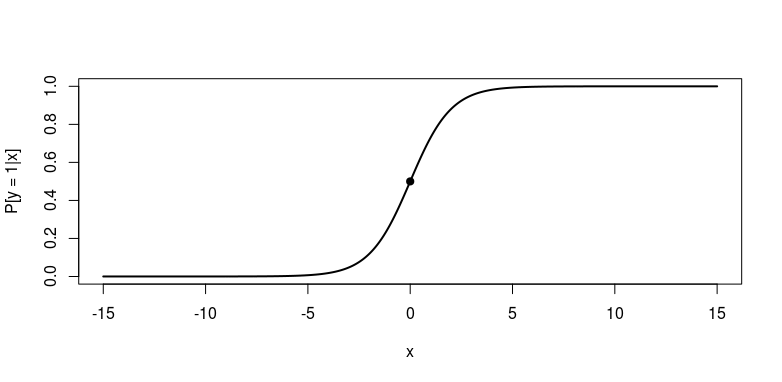
\includegraphics[width = 0.9\textwidth]{logistic_function.png}
	\caption{Logistic regression through the origin; $\beta = 1$.}
	\label{fig:logistic}
\end{figure}


% Problem 5
\subsection*{Problem 5: ANOVA -- with interactions without}

Key ideas/tools:
\begin{itemize}
\item calculations with the linear model
\end{itemize}

Here we present two solutions. The first uses vectorized notation, the second works with the coordinates. 
 
\subsubsection*{Vectorized solutions}

Let $\ones_I$ and $\ones_J$ represent the vectors of all $1$'s in dimensions $I$ and $J$ respectively. The ``outer product'' $\ones_I\ones_J^\top $ is a matrix in $\reals^{I \times J}$ of all $1$'s. We will think of $Y = (Y_{ij})$ as an element of $\reals^{I \times J}$. The given model can be written as 
\[Y = \mu \ones_I \ones_J^\top  + \alpha \ones_J^\top  + \ones_J \beta^\top  + \gamma + e, \]
where $e \in \reals^{I \times J}$ has i.i.d. entries with mean 0 and variance $\sigma^2$. The constraints on $\alpha,\beta$ and $\gamma$ can be written in vector notation,
\begin{align*}
	\alpha^\top  \ones_I&=0,\\
	\beta^\top  \ones_J&=0,\\
	\gamma \ones_J &= 0,\\
	\gamma^\top  \ones_I &=0.
\end{align*}
In particular, $\gamma$ is orthogonal to the space of main affects 
\begin{equation}\label{eq:subspace}U = \{\mu\ones_I\ones_J^\top  + \alpha \ones_J^\top  +\ones_I\beta^\top  \} \subseteq \reals^{I \times J}. \end{equation}
With this notation we will continue the question.
\begin{enumerate}
	\item[(a)] In this model, the OLS estimate of $\mu$ is the grand mean,
	\[\hat{\mu}=\bar{Y}_{+,+}=\frac{1}{IJ}\sum_{i=1}^I\sum_{j=1}^J Y_{i,j} = \frac{1}{IJ} \ones_I^\top  Y \ones_J. \]
	The OLS estimate of $\alpha$ is
	\[\hat{\alpha}_i = \bar{Y}_{i,+}-\bar{Y}_{+,+},  \]
	where $\bar{Y}_{i,+}$ is the group mean for level $i$. That is, 
	\[\bar{Y}_{i,+} = \frac{1}{J}\sum_{j=1}^J Y_{i,j}=\frac{1}{J}\left(Y\ones_J\right)_i .\] 
	We can calculate the expectation of $\bar{Y}_{i,+}$
	\begin{align*}
		\mathbb{E}[\bar{Y}_{i,+}]&=\frac{1}{J}\sum_{j=1}^J \bbE[Y_{i,j}]\\
		&=\frac{1}{J}\sum_{j=1}^J \mu+\alpha_i+\beta_j +\gamma_{ij} + \bbE[e_{ij}]\\
		&=\mu+\alpha_i,
	\end{align*}
	since $\beta_j^\top  \ones_J = 0$, $\gamma \ones_J=0$ and $\bbE[e_{ij}]=0$. By a similar calculation, the expectation of $\bar{Y}_{+,+}$ is $\mu$ and thus,
	\[\bbE[\hat{\alpha}_i] = \bbE[Y_{i,+}] - \bbE[\bar{Y}_{+,+}] = \mu +\alpha_i - \mu = \alpha_i. \]
	Thus,
	\[\bbE[\hat{\alpha}_i-\hat{\alpha}_{i'}] = \alpha_i-\alpha_{i'}, \]
	so the OLS estimate for $\alpha_i-\alpha_{i'}$ is unbiased.
	\item[(b)] Let $\hat{Y} \in \reals^{I\times J}$ be the fitted values in the main affects model. The main effects model has $I+J-1$ degrees of freedom (there are $I+J+1$ parameters and $2$ constraints). The usual estimate $\hat{\sigma}^2$ is thus
	\[\hat{\sigma}^2 = \frac{1}{IJ-(I+J-1)}\Vert Y - \hat{Y} \Vert_F^2 = \frac{1}{(I-1)(J-1)}\Vert Y - \hat{Y}_F^2 \]
	where $\Vert \cdot \Vert_F$ is the Frobenius norm on $\reals^{I \times J}$. Let $H$ be the projection onto the subspace $U$ from \eqref{eq:subspace}. We thus have,
	\begin{align*}
		Y-\hat{Y}&=(I-H)Y\\
		&=(I-H)(\mu\ones_I\ones^\top _J + \alpha\ones_J^\top  + \ones_I\beta^\top  +\gamma + e)\\
		&=\gamma + (I-H)e.
	\end{align*}
	The last line holds because by definition the main effects $\mu\ones_I\ones^\top _J + \alpha\ones_J^\top  + \ones_I\beta^\top $ are in $U$ and because $\gamma$ is orthogonal to $U$. Note that the rank of $(I-H)$ is exactly $IJ-(I+J+1)=(I-1)(J-1)$ and thus,
	\begin{align*}
		\bbE[\hat{\sigma}^2]&=\frac{1}{(I-1)(J-1)}\bbE[\Vert \gamma + (I-H)e\Vert_F^2]\\
		&=\frac{1}{(I-1)(J-1)}\bbE\left[\Vert \gamma \Vert_F^2 + 2\gamma^\top  (I-H)e + \Vert (I-H)e\Vert_F^2 \right] \\
		&=\frac{1}{(I-1)(J-1)}\left(\Vert \gamma \Vert_F^2 + (I-1)(J-1)\sigma^2\right)\\
		&=\sigma^2 + \frac{\Vert \gamma \Vert_F^2}{(I-1)(J-1)}.
	\end{align*}
	That is $\hat{\sigma}^2$ is biased upwards by,
	\[\frac{1}{(I-1)(J-1)} \Vert \gamma \Vert_F^2 = \frac{1}{(I-1)(J-1)}\sum_{i=1}^I\sum_{j=1}^J \gamma_{ij}^2 \ge 0. \]
	If we make the additional assumption that $e_{ij} \simiid \mathcal{N}(0,\sigma^2)$, then we can identify the distribution of $\hat{\sigma}^2$. By the above calculations we have 
	\[Y-\hat{Y} \sim \mathcal{N}_{I \times J}(\gamma, \sigma^2(I-H)), \]
	thus 
	\[\hat{\sigma}^2 = \frac{1}{(I-1)(J-1)}\Vert Y-\hat{Y}\Vert_F^2 \sim \frac{\sigma^2}{(I-1)(J-1)} \chi^2_{(I-1)(J-1)}(\Vert \gamma \Vert_F^2).\] 
	That is $\hat{\sigma}^2$ is a scaled non-central $\chi^2$ distribution.
	\item[(c)] As seen above
	\[\hat{\alpha}_2 - \hat{\alpha}_1 = \bar{Y}_{2,+} - \bar{Y}_{1,+} = \frac{1}{2}\left(Y_{2,1}+Y_{2,2}\right) - \frac{1}{2}\left(Y_{1,1}+Y_{1,2}\right), \]
	is unbiased of $\alpha_2 - \alpha_1$. Thus, we can $\alpha_1 - \alpha_2$ is identifiable. 
\end{enumerate}


\subsubsection*{Coordinate solution}

\begin{itemize}
\item[(a)] In fact, the usual least squares estimates of $\alpha_i$ are unbiased. Indeed,
		\begin{equation}
		\begin{split}
		\mathbb E[\hat \alpha_i] &= \mathbb E[\overline Y_{i+} - \overline Y_{+ +}] \\
		&= \mathbb E\left[\frac{1}{J}\sum_{j = 1}^J (\mu + \alpha_i + \beta_j + \gamma_{ij} + e_{ij}) - \frac{1}{IJ}\sum_{i = 1}^I \sum_{j = 1}^{J}(\mu + \alpha_i + \beta_j + \gamma_{ij} + e_{ij}) \right] \\
		&= \mu + \alpha_i - \mu \\
		&= \alpha_i
		\end{split}
		\end{equation}

Thus, the usual least squares estimates of $\alpha_i - \alpha_{i'}$ will also be unbiased.

\item[(b)] Note that 
\begin{align*}
\hat{\mu} &= \frac{1}{IJ} \sum_{i,j} Y_{ij} = \frac{1}{IJ}\sum_{i,j} (\mu +  e_{ij}) = \mu + \overline e_{+ +}, \\ 
\hat{\alpha_i} &= \frac{1}{J} \sum_j Y_{ij} - \frac{1}{IJ} \sum_{i,j} Y_{ij} = \alpha_i + \overline e_{i +} - \overline e_{+ +}, \\
\hat{\beta_j} &= \frac{1}{I} \sum_i Y_{ij} - \frac{1}{IJ} \sum_{i,j} Y_{ij} = \beta_j + \overline e_{+ j} - \overline e_{+ +}.
\end{align*}

Thus, we have
		\begin{equation*}
		\begin{split}
		\mathbb E[\hat \sigma^2] &= \mathbb E\left[\frac{1}{(I-1)(J-1)}\sum_{i = 1}^I \sum_{j = 1}^J (Y_{ij} - \hat \mu - \hat \alpha_i - \hat \beta_j)^2\right] \\
		&= \mathbb E\left[\frac{1}{(I-1)(J-1)}\sum_{i = 1}^I \sum_{j = 1}^J (\gamma_{ij} + e_{ij} - \overline e_{i+} - \overline e_{+ j} + \overline e_{+ +})^2\right] \\
		&= \frac{1}{(I-1)(J-1)}\sum_{i = 1}^I \sum_{j = 1}^J \mathbb E\left[(\gamma_{ij} + e_{ij} - \overline e_{i+} - \overline e_{+ j} + \overline e_{+ +})^2\right] \\
		&= \mathbb E\left[\frac{1}{(I-1)(J-1)}\sum_{i = 1}^I \sum_{j = 1}^J (e_{ij} - \overline e_{i+} - \overline e_{+ j} + \overline e_{+ +})^2\right] + \frac{1}{(I-1)(J-1)}\sum_{i = 1}^I \sum_{j = 1}^J \gamma_{ij}^2 \\
		&= \sigma^2 + \frac{1}{(I-1)(J-1)}\sum_{i = 1}^I \sum_{j = 1}^J \gamma_{ij}^2.
		\end{split}
		\end{equation*}
		The last equality holds because the quantity in brackets in the penultimate line is the unbiased estimate for $\sigma^2$ in the no-interactions model. Hence, we find that $\hat \sigma^2$ is biased upwards for $\sigma^2$. This will have the effect of deflating the significance of $F$ tests for $\alpha_1 = \cdots = \alpha_I$ and $\beta_1= \cdots = \beta_J$. 
		
		Another way to see that the last line above holds is to use linearity of expectation and to note that since $e_{ij} \stackrel{\text{IID}}{\sim} N(0,\sigma^2)$, then for each $i,j$, $$\begin{bmatrix} e_{ij} \\  \overline e_{i +} \\ \overline e_{+ j} \\  \overline e_{+ +}  \end{bmatrix} \sim \mathcal{N} \Bigg( \begin{bmatrix} 0 \\  0 \\ 0 \\  0  \end{bmatrix}, \sigma^2 \begin{bmatrix} 1  & \frac{1}{J} & \frac{1}{I} & \frac{1}{IJ} \\ \frac{1}{J} & \frac{1}{J} & \frac{1}{IJ}  &  \frac{1}{IJ} \\ \frac{1}{I} & \frac{1}{IJ} & \frac{1}{I} &  \frac{1}{IJ} \\ \frac{1}{IJ} &  \frac{1}{IJ} &  \frac{1}{IJ} & \frac{1}{IJ}  \end{bmatrix}  \Bigg)$$ and hence letting $v=(1,-1,-1,1)$,  $$e_{ij} - \overline e_{i+} - \overline e_{+ j} + \overline e_{+ +} \sim \mathcal{N} \Bigg(0, \sigma^2 v^\top   \begin{bmatrix} 1  & \frac{1}{J} & \frac{1}{I} & \frac{1}{IJ} \\ \frac{1}{J} & \frac{1}{J} & \frac{1}{IJ}  &  \frac{1}{IJ} \\ \frac{1}{I} & \frac{1}{IJ} & \frac{1}{I} &  \frac{1}{IJ} \\ \frac{1}{IJ} &  \frac{1}{IJ} &  \frac{1}{IJ} & \frac{1}{IJ}  \end{bmatrix} v \Bigg) = \mathcal{N}\big( 0, \sigma^2 (1 -\frac{1}{J} -\frac{1}{I} + \frac{1}{IJ} ) \big),$$ so indeed $$\frac{1}{(I-1)(J-1)}\sum_{i = 1}^I \sum_{j = 1}^J  \mathbb{E} \left[ (e_{ij} - \overline e_{i+} - \overline e_{+ j} + \overline e_{+ +})^2\right] =\sigma^2.$$

\item[(c)] A direct way of checking identifiability is to note that

$$ \EE{ \frac{Y_{11}  + Y_{12}}{2} - \frac{Y_{21}  + Y_{22}}{2}} = \alpha_1 - \alpha_2. $$

\end{itemize}



% Problem 6
\subsection*{Problem 6: Testing linearity with replicates}
Key ideas/tools:
\begin{itemize}
\item F-test
\item residual bootstrap
\end{itemize}
\begin{itemize}
\item[(a)] Given i.i.d. normal errors, we can use the $F$ test to compare 
	\begin{equation}
	H_0: y_{ij} = \beta_0 + \beta_1 x_i + e_{ij} \quad \text{vs.} \quad H_1: y_{ij} = \sum_{i' = 1}^k \beta_{i'} I(x_i = x_{i'}) + e_{ij}.
	\end{equation}
	Here, $H_0$ represents the linear model and $H_1$ represents the saturated model.
	The resulting F statistic is
	\begin{equation}
	F = \frac{\frac{1}{k - 2}\sum_{i, j}(\overline y_{i\cdot} - \hat \beta_0 - \hat \beta_1 x_i)^2}{\frac{1}{km-k}\sum_{i, j}(y_{ij} - \overline y_{i\cdot})^2}.
	\label{F}
	\end{equation}
	This is the ratio of the ``lack of fit sum of squares" to the ``pure error sum of squares," and has a null distribution of $F_{k-2, km-k}$.

\item[(b)] The main idea here is to describe some sort of bootstrap test. However, there are many possible ways to set this up. Here are the solutions that have acculated over the years.

\textbf{Solution 1:} Suppose that $y_{ij} = m(x_i) + e_{ij}$, where $e_{ij} \overset{\text{i.i.d.}}\sim F$ for some unknown error distribution $F$ with mean $0$.  A reasonable approach here is to bootstrap residuals. In particular let $\hat{e}_{ij} =  y_{ij} - \hat{\beta}_0 - \hat{\beta}_1x_i$. Then, we can generate bootstrap datasets by setting
\[
	y_{ij}^* = \hat \beta_0 + \hat \beta_1 x_{i} + \hat{e}_{ij}^*
\]
where $\hat{e}_{ij}^*$ are sampled with replacement from the set $\{\hat e_{ij}\}$. We can then recalculate the $F$ statistic (\ref{F}) for each bootstrapped data set and thereby generate its null distribution.\\

I think it is instructive to also consider the solution of a previous coach who suggested to use the same procedure, but with $\hat{e}_{ij}  = y_{ij} - \bar{y}_{i\cdot}$. Note that in this case $\hat{e}_{ij} = e_{ij} - \bar{e}_{i \cdot}$. If $m$ is small the empirical distribution of $\hat{e}_{ij}$ may not be very close to $F$ and thus we probably should not expect this procedure to work. On the other hand, if $m$ is large this is likely also valid.\\  
    
If we think that the error distribution changes with $x$ (e.g. if there is heteroskedasticity), then we can also resample the residuals separately for each $x$. However, this will also probably only work when $m$ is large.

A previous coach also suggested that when $m$ is large, we may still trust using the F-test from part (a), if $m$ is large enough for the Central Limit Theorem has kicked in. Typically we expect the Central Limit Theorem to kick in whenever $n \gg p$ or equivalently in this case when $m \gg 1$. However, while I see how the Central Limit Theorem can kick in for the numerator of the $F$-statistic as $m \to \infty$, I don't quite see how in the limit as $m \to \infty$ the central limit theorem would kick in for the denominator and make it approximately $\chi_{km-k}^2$.

\textbf{Alternative solutions when $m$ is fixed $k \to \infty$:} An alternative solution is to explicitly evaluate the limiting distribution of the F-statistics. Let $X \in \mmr^{m k \times 2}$ be the design matrix with rows $X_1,\dots,X_{m k }$. Write
\begin{align*}
F = \frac{km-k}{k-2} \left( \frac{y^\top (I-X(X^\top X)^{-1}X^\top )y}{\sum_{i,j}(e_{ij} - \bar{e}_{i \cdot})^2} - 1 \right) = \frac{km-k}{k-2} \left( \frac{e^\top (I-X(X^\top X)^{-1}X^\top )e}{\sum_{i,j}(e_{ij} - \bar{e}_{i \cdot})^2} - 1 \right) 
\end{align*}
Without loss of generality assume that the second column of $X$ is centred and both columns are scaled so that $X^\top X = I$. Then,
\begin{align*}
F & =  \frac{km-k}{k-2} \left( \frac{e^\top e - ||\sum_{i,j} x_i e_{ij}||^2   }{\sum_{i,j}(e_{ij} - \bar{e}_{i \cdot})^2} - 1 \right)\\
&  =  \frac{km-k}{k-2} \left(\frac{m\sum_{i} (\bar{e}_{i\cdot})^2  }{\sum_{i,j}e_{ij}^2 - (\bar{e}_{i \cdot})^2}  \right) - O_P(1/k)\\
& =  \frac{km-k}{k-2} \left(\frac{m^{-1}\sum_{i,j} e_{ij}^2  +  m^{-1}\sum_{i} \sum_{j \neq j'} e_{ij}e_{ij'}  }{(1-1/m)\sum_{i,j}e_{ij}^2 - (1/m) \sum_{j \neq j'} e_{ij} e_{ij'}  }  \right) - O_P(1/k)
\end{align*}
So, we find that 
\begin{align*}
\sqrt{k}\left(F - \frac{k}{k-2}\right) & = \sqrt{k} \frac{k}{k-2} \left(\frac{m^{-1}\sum_{i,j} e_{ij}^2  + m^{-1} \sum_{i} \sum_{j \neq j'} e_{ij}e_{ij'}  }{  m^{-1} \sum_{i,j}e_{ij}^2 - m^{-1}(m-1)^{-1} \sum_{j \neq j'} e_{ij} e_{ij'}  } - 1 \right) - O_P(1/k)\\
& = \sqrt{k} \frac{k}{k-2} \left(   \frac{  (m-1)^{-1} \sum_{i} \sum_{j \neq j'} e_{ij}e_{ij'} }{  m^{-1} \sum_{i,j}e_{ij}^2 - m^{-1}(m-1)^{-1} \sum_{j \neq j'} e_{ij} e_{ij'}  }    \right) - O_P(1/k)\\
& \stackrel{D}{\to} N(0, 2m(m-1))
\end{align*}
Note that the limiting distribution does not depend on the distribution of the errors and in particular the limiting distribution when $e_{ij} \sim N(0,\sigma^2)$ is the same as the limiting distribution in the case where $e_{ij} \sim F$ for $F$ an arbitrary distribution with a finite second moment. Thus, the F-test proposed in part a will be accurate without needing to assume normality. 



\item[(c)] If there had been no replication, then the denominator of the $F$ statistic would be zero, i.e. the $F$ test would not be valid. Hence, we need to make our saturated model a little less saturated. For example, if Engineer A sees a polynomial-looking relationship between $y$ and $x$, then one could do an $F$ test versus a larger model with some higher-order terms in $x$. Bootstrapping residuals could also work in this case. 

If we have densely spaced covariate values $x_i$, another approach we could take is to approximate the lack of fit $F$ test by simply grouping points with similar $x_i$. In general, this approach will underestimate the difference between $x_i^\top \beta$ and $m(x_i)$ and thus will produce a conservative test.

\item[(d)] We would question the independence of errors across $i$ if $i$ indexed space or time. We know that spatial and temporal data often exhibit local correlations in errors. We would question the independence of $e_{ij}$ across $j$ if there were systematic differences in the data collection process across $i$, e.g. if $i$ indexes days and a different person collected the data on each day. This would introduce positive correlations among $e_{ij}$ for each $i$, which would inflate our $F$ statistics by underestimating their denominators.

\end{itemize}
